\section{Постановка задачи}

Вычислить интервальные оценки параметров распределения, определить доверительные интервалы для оценки неизвестных параметров нормального распределения: математического ожидания и дисперсии.

\section{Ход работы}

В ходе работы была сгенерирована генеральная совокупность (<<data>>) из 200 значений нормально распределённой случайной величины со случайными параметрами матиематического ожидания и стандартного отклонения (указаны в консольном выводе в конце файла). Для смоделированной генеральной совокупности были построены гистограмма и полигон относительных частот для 8 и 12 интервалов разбиения:

\begin{figure}[H]
	\begin{minipage}[H]{0.49\linewidth}
		\begin{center}
			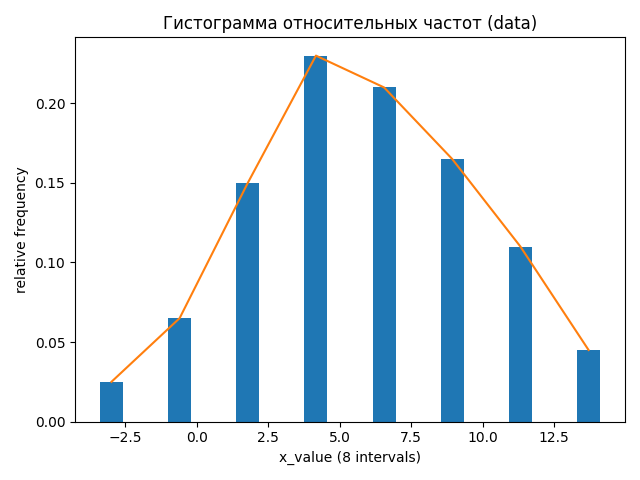
\includegraphics[width=\linewidth]{figures/rel_freq_hist_8_bins_data}
		\end{center}
	\end{minipage}
	\hfill
	\begin{minipage}[H]{0.49\linewidth}
		\begin{center}
			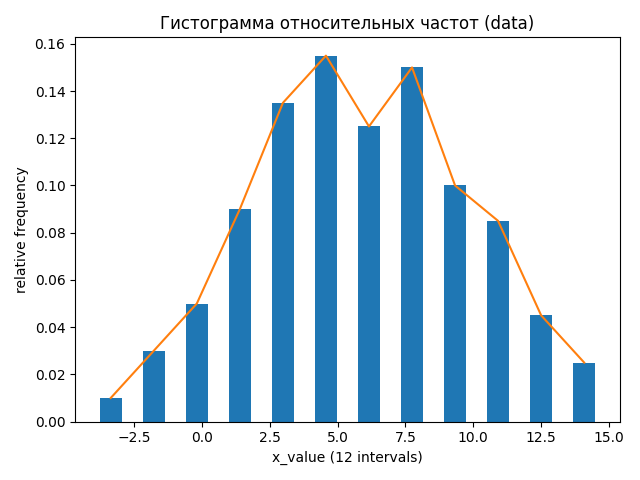
\includegraphics[width=\linewidth]{figures/rel_freq_hist_12_bins_data}
		\end{center}
	\end{minipage}
\end{figure}

Также были вычислены дисперсия, стандартное отклонение и математическое ожидание полученной генеральной совокупности.

Найдены вероятности попадания случайной величины $X \in  N(a, \sigma^2)$ в интервал $[5;11]$ по следующей формуле:

\begin{equation}
	P\{5 < X < 11\} = F(11) - F(5),
\end{equation}
где $F(x)$ - функция Гаусса. Были получены 2 вероятности: одна вычислена по искомым значениям $a$ и $\sigma$, а вторая - по полученным из генеральной совокупности. Абсолютная разность этих вероятностей отличается в 3ем знаке после запятой, что говорит о значительной близости результатов, и, как следствие, схожести полученных параметров с исходными.

Далее были сформированы 2 выборки (<<sample1>> и <<sample2>>) объёмом 30 элементов, которые были получены случайным отбором из генеральной совокупности. Для каждой выборки построены точечные оценки параметров распределения, а также были построены гистограммы относительных частот для 5 и 7 интервалов разбиения:

\begin{figure}[H]
	\begin{minipage}[H]{0.45\linewidth}
		\begin{center}
			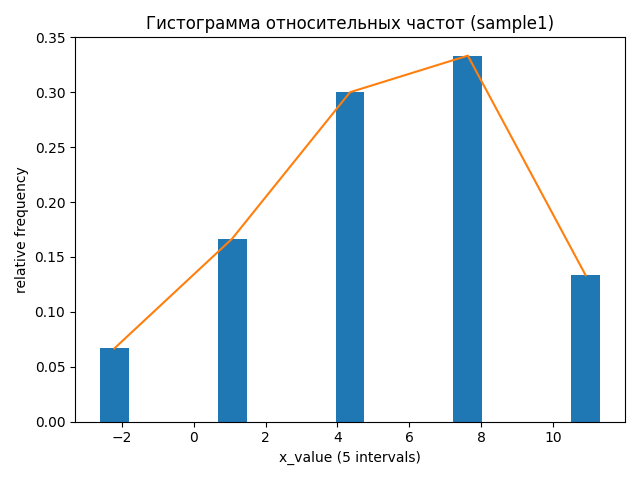
\includegraphics[width=\linewidth]{figures/rel_freq_hist_5_bins_sample1}
		\end{center}
	\end{minipage}
	\hfill
	\begin{minipage}[H]{0.45\linewidth}
		\begin{center}
			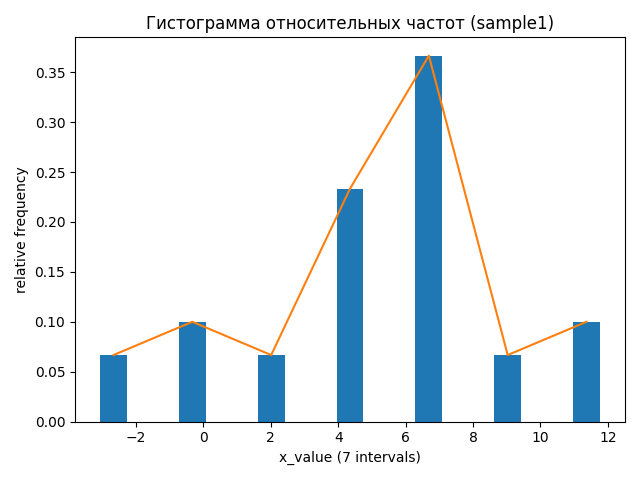
\includegraphics[width=\linewidth]{figures/rel_freq_hist_7_bins_sample1}
		\end{center}
	\end{minipage}
	\vfill
	\begin{minipage}[H]{0.45\linewidth}
		\begin{center}
			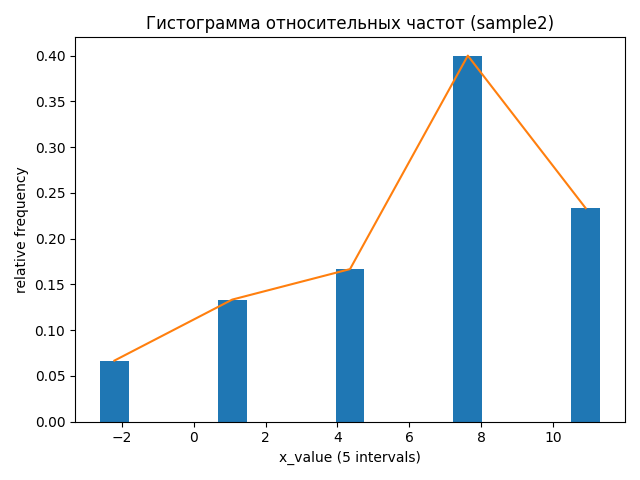
\includegraphics[width=\linewidth]{figures/rel_freq_hist_5_bins_sample2}
		\end{center}
	\end{minipage}
	\hfill
	\begin{minipage}[H]{0.45\linewidth}
		\begin{center}
			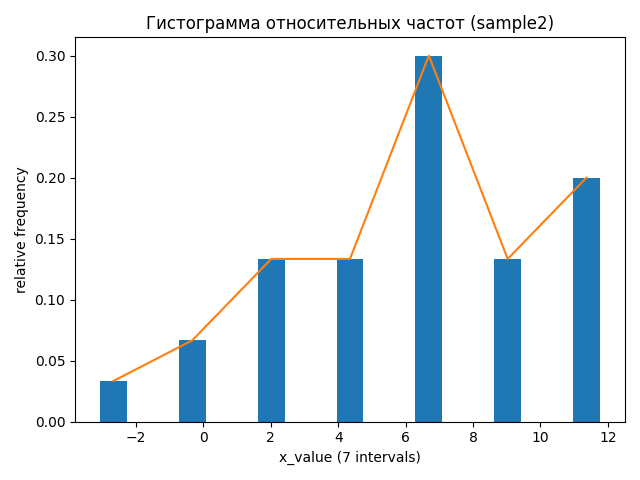
\includegraphics[width=\linewidth]{figures/rel_freq_hist_7_bins_sample2}
		\end{center}
	\end{minipage}
\end{figure}

Наконец, для генеральной совокупности и 2х выборок были вычислены следующие доверительные интервалы (везде уровень значимости равен 5\%):

\begin{itemize}
	\item Доверительный интервал для оценки неизвестного математического ожидания

	\begin{equation}
		\overline{x_0} - z_{table} \frac{\sigma}{\sqrt{n}} < a < \overline{x_0} + z_{table} \frac{\sigma}{\sqrt{n}},
	\end{equation}
	где $z_{table}$ - квантиль нормального распределения.

	\item Доверительный интервал для оценки математического ожидания при неизвестном значении генерального среднеквадратического отклонения:

	\begin{equation}
		\overline{x_0} - t_{table} \frac{\tilde{S}}{\sqrt{n}} < a < \overline{x_0} + t_{table} \frac{\tilde{S}}{\sqrt{n}},
	\end{equation}
	где $t_{table}$ - квантиль расределения Стьюдента с $n - 1$ степенью свободы.

	\item Доверительный интервал для оценки дисперсии при неизвестном значении генерального среднего:

	\begin{equation}
		\frac{(n-1)\tilde{S^2}}{t_2} \leq \sigma^2 \leq \frac{(n-1)\tilde{S^2}}{t_1},
	\end{equation}
	где $t_1, t_2$ - квантили распределения Пирсона $\tilde{\chi^2}$ с $n - 1$ степенью свободы.

	\item Доверительный интервал для оценки среднеквадратичного отклонения при неизвестном значении генерального среднего

	\begin{equation}
		\frac{\sqrt{n-1}\tilde{S}}{\sqrt{t_2}} \leq \sigma \leq \frac{\sqrt{n-1}\tilde{S}}{\sqrt{t_1}},
	\end{equation}
	где $t_1, t_2$ - квантили распределения Пирсона $\tilde{\chi^2}$ с $n - 1$ степенью свободы.

\end{itemize}

Добавочным заданием было нахождение доверительного интервала с уровнем значимости 5\% для параметра $p$ из распределения Бернулли, пользуясь интегральной предельной теоремой Муавра-Лапласа. Изначально была сгенерирована выборка из распределения Бернулли объёма 500 и выбрано значение $p = 0.3$. Далее, необходимо воспользоваться формулой, асимптотически описывающая доверительный интервал для вероятности $p$:

\begin{equation}
	\left(\frac{m}{n} - z_{1 - \frac{\alpha}{2}} \frac{\sqrt{\frac{m}{n} \left(1 - \frac{m}{n} \right)}}{\sqrt{n}},
	\frac{m}{n} + z_{1 - \frac{\alpha}{2}} \frac{\sqrt{\frac{m}{n} \left(1 - \frac{m}{n} \right)}}{\sqrt{n}} \right),
\end{equation}
где $m$ - число единиц, $n$ - общее число испытаний, $z_{1 - \frac{\alpha}{2}}$ - квантиль стандартного нормального распределения.

Все численные результаты, полученные в ходе выполнения работы, представлены ниже.

\VerbatimInput{figures/file.txt}
